\subsection{PHY driver and link management}

\begin{frame}{PHY devices}
	\begin{columns}
		\column{0.35\textwidth}
		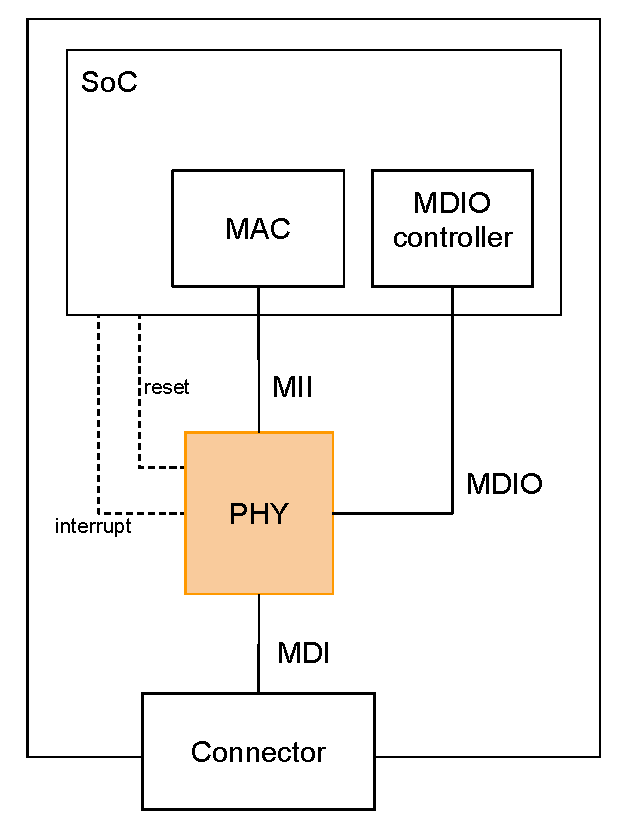
\includegraphics[width=\textwidth]{slides/networking-driver-phy/phy_easy.pdf}
		\column{0.65\textwidth}
		\begin{itemize}
			\item Ethernet PHYs handle Layer 1 of the OSI model
			\item Standardised by IEEE 802.3
			\item \textbf{M}edia \textbf{I}ndependent \textbf{I}nterface
				\begin{itemize}
					\item Communication bus between MAC and PHY
				\end{itemize}
			\item \textbf{M}edia \textbf{D}ependent \textbf{I}nterface
				\begin{itemize}
					\item Communication medium with the \textbf{link partner}
					\item Can be Cat6 cable, Fibre, Coax, backplane, etc.
				\end{itemize}
			\item \textbf{M}anagement \textbf{D}ata \textbf{I}nput \textbf{O}utput
				\begin{itemize}
					\item Control bus for PHY devices
					\item Can be shared by multiple PHYs
					\item Allows accessing PHY registers
				\end{itemize}
			\item Optionally, PHYs can raise interrupts
				\begin{itemize}
					\item \textit{e.g.} to report link status change
				\end{itemize}
			\item Optionally, PHYs can have a reset line


		\end{itemize}
	\end{columns}
\end{frame}

\begin{frame}{MDIO Bus}
	\hfill
	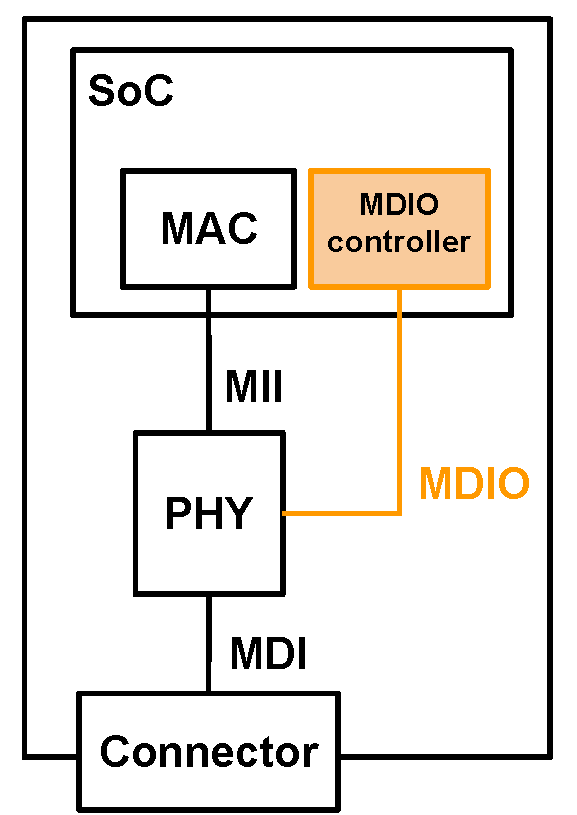
\includegraphics[width=0.15\textwidth]{slides/networking-driver-phy/mdio.pdf}
	\vspace{-3cm}
	\begin{itemize}
		\item Most common bus to access Ethernet PHYs
		\item Addressable, 32 addresses
		\item Physically very similar to i2c
			\begin{itemize}
				\item An \textbf{adapter} initiates all transfers to \textbf{devices} 
				\item 2 physical signals : \textbf{MDC} for the clock, \textbf{MDIO} for data
			\end{itemize}
		\item 802.3 defines 2 protocols for MDIO :
			\begin{itemize}
				\item Clause 22 : 5 bits device address, 5 bits register address, 16 bits data
				\item Clause 45 : 3-part addresses : 5 bits addresses, 5 bits \textbf{devtype}, 16 bits register address, 16 bits data
				\item \textbf{devtype} allows addressing sub-components of the PHY : PCS, PMA/PMD, etc.
				\item C45 is backwards compatible with C22
			\end{itemize}
		\item Register layout is defined by \textbf{802.3}, with room for vendor-specific registers
		\item a \href{https://elixir.bootlin.com/linux/v6.15.1/source/drivers/net/mdio/mdio-bitbang.c}{gpio bitbang} MDIO driver exists
	\end{itemize}
\end{frame}

\begin{frame}[fragile]{MDIO driver}
	\begin{itemize}
		\item MDIO controller drivers are represented by \kstruct{mii_bus}
		\item Contains callback ops for \code{C22} and \code{C45} access :
	\end{itemize}
	\vspace{0.5cm}
	{\fontsize{9}{10}
	\begin{minted}{c}
struct mii_bus {
        const char *name;
        void *priv;
        int (*read)(struct mii_bus *bus, int addr, int regnum);
        int (*write)(struct mii_bus *bus, int addr, int regnum, u16 val);
        int (*read_c45)(struct mii_bus *bus, int addr, int devnum, int regnum);
        int (*write_c45)(struct mii_bus *bus, int addr, int devnum, int regnum, u16 val);
        int (*reset)(struct mii_bus *bus);
/* ... truncated ... */
};
	\end{minted}
	}
\end{frame}

\begin{frame}[fragile]{MDIO accessors}
	\begin{itemize}
		\item Raw read/write operations :
			{\fontsize{9}{10}
			\begin{minted}{c}
int mdiobus_read(struct mii_bus *bus, int addr, u32 regnum);
int mdiobus_write(struct mii_bus *bus, int addr, u32 regnum, u16 val);
int mdiobus_c45_read(struct mii_bus *bus, int addr, int devad, u32 regnum);
int mdiobus_c45_write(struct mii_bus *bus, int addr,  int devad, u32 regnum, u16 val);
			\end{minted}
			}
		\item Wrapped by phylib for convenience : \kfunc{phy_read}, \kfunc{phy_read_mmd}, etc.
		\item Unlocked versions : \kfunc{__mdiobus_write}, \kfunc{__phy_write}, etc.
			\begin{itemize}
				\item Caller implements their own locking
				\item Useful for large transfers, \textit{e.g.} loading a firmware
			\end{itemize}
	\end{itemize}
\end{frame}

\begin{frame}{MDIO access from userspace}
	\begin{itemize}
		\item \code{ioctl} based API, limited on purpose
		\item Useful for debugging, but interferes with phylib
			\begin{itemize}
				\item Phylib and drivers have no way to track user-made configuration
			\end{itemize}
		\item Main userspace tool is \code{phytool}
			\begin{itemize}
				\item \code{phytool read eth0/1/2} : Read register 2 from mdio device at address 1
				\item \code{phytool read eth0/1:2/3} : Read register 3 on MMD 2 from mdio device at address 1
			\end{itemize}
		\item Can be tedious for indirect accesses
		\item \textbf{mdio-tools} uses an out-of-tree module to access MDIO over Netlink
	\end{itemize}
\end{frame}

\begin{frame}[fragile]{MDIO controllers in devicetree}
	\begin{columns}
		\column{0.5\textwidth}
		\begin{block}{\kfile{arch/arm64/boot/dts/marvell/armada-37xx.dtsi}}
		{\fontsize{9}{10}
			\begin{minted}{perl}
mdio: mdio@32004 {
    #address-cells = <1>;
    #size-cells = <0>;
    compatible = "marvell,orion-mdio";
    reg = <0x32004 0x4>;
};
			\end{minted}
		}
		\end{block}

		\begin{block}{\kfile{arch/arm/boot/dts/st/stm32mp15xx-dkx.dtsi}}
			{\fontsize{9}{10}
			\begin{minted}{perl}
&ethernet0 {
    mdio {
        compatible = "snps,dwmac-mdio";
        /* ... */
    };
};
			\end{minted}
			}
		\end{block}
		\column{0.5\textwidth}
		\begin{itemize}
			\item SoCs may have dedicated MDIO controllers
				\begin{itemize}
					\item Dedicated drivers with their own \code{compatible}
				\end{itemize}
			\item Some MACs and DSA switches have an integrated MDIO controller
				\begin{itemize}
					\item \code{mdio} child node within the MAC controller's node
				\end{itemize}
		\end{itemize}
	\end{columns}
\end{frame}

\begin{frame}[fragile]{Ethernet PHYs identification}
	\begin{itemize}
		\item 802.3 specifies that registers 0x2 and 0x3 are \textbf{identifiers}
			\begin{itemize}
				\item \code{OUI} (24 bits) and \code{Model} information (10 bits)
			\end{itemize}
		\item PHY drivers register which identifier they support
			\begin{itemize}
				\item \code{phy_driver.phy_id}
			\end{itemize}
		\item We don't need per-device \code{compatible} strings in devicetree
		\item PHY \code{compatible} is used to indicate :
			\begin{itemize}
				\item The MDIO clause :
					\begin{itemize}
						\item \code{ethernet-phy-ieee802.3-c22}
						\item \code{ethernet-phy-ieee802.3-c45}
					\end{itemize}
				\item The PHY id, if PHY reports the wrong information
					\begin{itemize}
						\item \textit{e.g.} \code{ethernet-phy-id2000.a231}
					\end{itemize}
			\end{itemize}
	\end{itemize}
\end{frame}

\begin{frame}[fragile]{Ethernet PHYs in devicetree}
	\begin{columns}
		\column{0.55\textwidth}
		\begin{block}{\kfile{arch/arm64/boot/dts/marvell/armada-8040-mcbin.dtsi}}
		{\fontsize{9}{10}
			\begin{minted}{perl}
&cp0_mdio {
    status = "okay";
    
    ge_phy: ethernet-phy@0 {
        reg = <0>;
    };
};

&eth0 {
        phy-handle = <&ge_phy>;
}
			\end{minted}
		}
		\end{block}
		\column{0.5\textwidth}
		\begin{itemize}
			\item \code{reg} - mandatory
				\begin{itemize}
					\item The PHY's address on the MDIO bus
					\item Usually assigned via PCB straps
				\end{itemize}
			\item \code{reset-gpios} : GPIO reset line
			\item \code{rx|tx-internal-delay-ps}
				\begin{itemize}
					\item RGMII delays adjustments
				\end{itemize}
			\item \code{leds} : LEDs driven by the PHY
			\item \code{interrupts} :
				\begin{itemize}
					\item Status interrupt, level-triggered
				\end{itemize}
			\item \code{sfp} : \textit{phandle} to an SFP cage description
		\end{itemize}
	\end{columns}

\end{frame}

\begin{frame}{PHY devices in the kernel}
	\hfill
	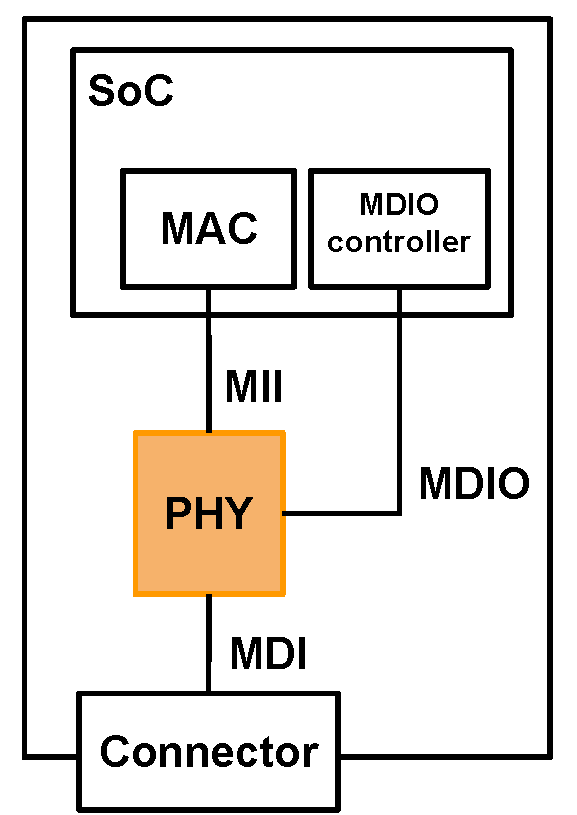
\includegraphics[width=0.15\textwidth]{slides/networking-driver-phy/phy.pdf}
	\vspace{-3cm}
	\begin{itemize}
		\item A PHY driver is represented by \kstruct{phy_driver}
		\item PHY instances are represented by \kstruct{phy_device}
			\begin{itemize}
				\item By convention, objects are named \code{phydev} or \code{phy}
			\end{itemize}
		\item \textbf{All} Ethernet PHY devices are \code{mdio} devices
			\begin{itemize}
				\item Fixed-PHY uses an \href{https://elixir.bootlin.com/linux/v6.15.1/source/drivers/net/phy/swphy.c}{emulated bus}
				\item Memory-mapped PHYs can use a \href{https://elixir.bootlin.com/linux/v6.15.1/source/drivers/net/mdio/mdio-regmap.c}{regmap conversion layer}
			\end{itemize}
		\item Managed by the \textbf{phylib} PHY framework
		\item PHY drivers mostly handle the vendor-specific aspects
		\item Most of the standardised logic is generic, and implemented in phylib
		\item A \href{https://elixir.bootlin.com/linux/v6.15.1/source/drivers/net/phy/phy_device.c\#L3510}{Generic driver} implements only the standard logic
			\begin{itemize}
				\item Used as a fallback when a PHY is detected with no associated driver
			\end{itemize}
	\end{itemize}
\end{frame}

\begin{frame}{PHY device role}
	\begin{itemize}
		\item The PHY driver reports the \textbf{link status} :
			\begin{itemize}
				\item Updated by \code{phy_driver.read_status()}
					\begin{itemize}
						\item Called upon PHY interrupt, or polled
					\end{itemize}
				\item \code{phydev.link} : Link with the partner is \code{UP} or \code{DOWN}
				\item \code{phydev.speed} : Established link speed, in Mbps
				\item \code{phydev.duplex} : Established duplex (half or full)
			\end{itemize}
		\item It is in charge of configuring and performing the \textbf{Link negociation}
			\begin{itemize}
				\item Based on what the MAC can do and user-specified parameters
				\item \textit{e.g.} \code{ethtool -s eth0 speed 100 duplex full autoneg on} on a 1G interface
			\end{itemize}
		\item It may implement some \textbf{offloaded operations}
			\begin{itemize}
				\item Some PHYs can offload \textbf{MACSec}
				\item PHY timestamping is implemented by some devices
			\end{itemize}
	\end{itemize}
\end{frame}

\begin{frame}{PHY device role - 2}
	\begin{itemize}
		\item \textbf{Wake on Lan} can be implemented at the PHY level
			\begin{itemize}
				\item The PHY receives the \href{https://en.wikipedia.org/wiki/Wake-on-LAN\#Magic_packet}{magic packet}
				\item It triggers an interrupt to wake the system up
				\item \code{phy_driver.set_wol()} and \code{phy_driver.get_wol()}
			\end{itemize}
		\item Some PHYs can perform \textbf{cable testing}
			\begin{itemize}
				\item Detects cable and connector faults
				\item \code{ethtool --cable-test eth0}
			\end{itemize}
		\item They may report stats, useful for debugging link bringup
			\begin{itemize}
				\item \code{ethtool --phy-statistics eth0}
			\end{itemize}
		\item \textbf{\code{BaseT1S}} PHYs can configure the \href{https://docs.kernel.org/networking/ethtool-netlink.html\#plca-get-cfg}{plca} parameters

	\end{itemize}
\end{frame}

\begin{frame}[fragile]{Fixed-link}
	\begin{itemize}
		\item The PHY is responsible for reporting the link state, but doesn't always exist
		\item \textit{e.g.} MAC to MAC links, between a SoC and a DSA switch
		\item Fixed-link allows describing a link that is always \code{UP}
		\item In creates a virtual PHY internally that reports fixed parameters
	\end{itemize}
	\begin{block}{fixed link example}
		\begin{minted}{perl}
&eth0 {
        /* ... */
        fixed-link {
                speed = <1000>;
                full-duplex;
        };
};
		\end{minted}
	\end{block}
\end{frame}

\begin{frame}{MII}
	\hfill
	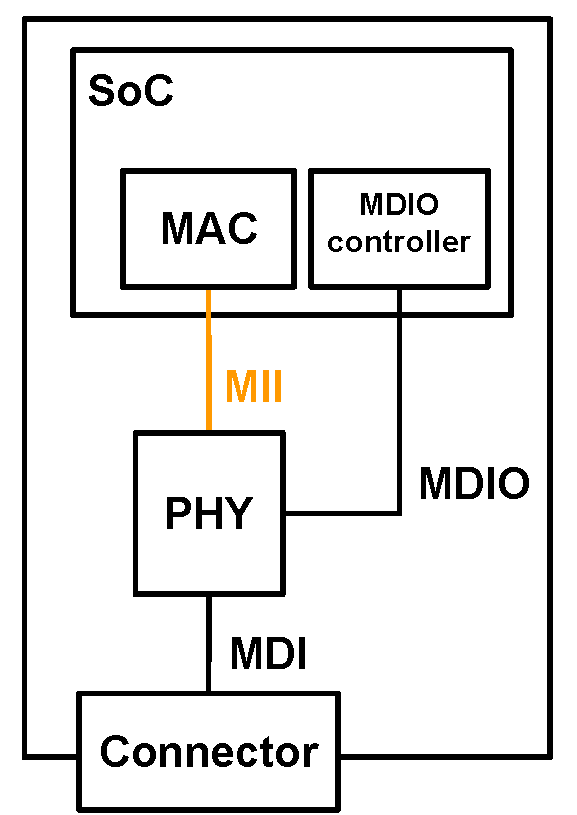
\includegraphics[width=0.15\textwidth]{slides/networking-driver-phy/mii.pdf}
	\vspace{-3cm}
	\begin{itemize}
		\item \textbf{M}edia \textbf{I}ndependent \textbf{I}nterface
		\item Conveys the data stream between MAC and PHY
		\item Specified in devicetree via \code{phy-mode} or \code{phy-connection-type}
		\item In some scenarios, the mode may change dynamically
			\begin{itemize}
				\item For \textbf{serialized} modes that are physically compatible
				\item Depending on the negociated link speed, the PHY may change its mode
				\item example: the \href{https://elixir.bootlin.com/linux/v6.15.1/source/drivers/net/phy/marvell10g.c}{Marvell 88x3310 PHY}
				\item When link speed is negociated at 1Gbps, uses \textbf{SGMII}
				\item When link speed is negociated at 2.5Gbps, uses \textbf{2500BaseX}
				\item When link speed is negociated at 10Gbps, uses \textbf{10GBaseR}
			\end{itemize}
		\item On the MAC side, may require spefific \textbf{PCS} and \textbf{Serdes} configuration
	\end{itemize}
\end{frame}

\begin{frame}{MII flavours - Parallel interfaces}
	\begin{itemize}
		\item \code{MII} : Also describes a 8-bit, 10/100Mbps interface
		\item \code{RMII} : \textbf{R}educed \textbf{MII} : 4 bits, 10/100Mbps
			\begin{itemize}
				\item Popular mode for 100Mbps interfaces
			\end{itemize}
		\item \code{GMII} : \textbf{G}igabit \textbf{MII} : 8 bits, 10/100/1000Mbps
			\begin{itemize}
				\item Rarely found on PCBs, mostly unsed within the SoC
			\end{itemize}
		\item \code{RGMII} : \textbf{R}educed \textbf{G}igabit \textbf{MII} : 4 bits, 10/100/1000Mbps
			\begin{itemize}
				\item Popular mode for 1Gbps interfaces
			\end{itemize}
		\item \code{XGMII} : \textbf{X} (Roman Numeral 10) \textbf{G}igabit \textbf{MII} : 32 bits, 10Gbps
		\item \code{XLGMII} : \textbf{XL} (Roman Numeral 40) \textbf{G}igabit \textbf{MII} : 32 bits, 40Gbps
			\begin{itemize}
				\item \textbf{XGMII} and \textbf{XLGMII} are on-silicon modes, not used on PCBs
			\end{itemize}
	\end{itemize}
\end{frame}

\begin{frame}{MII flavours - Serial interfaces}
	\center{Differential pairs for Data (1 RX + 1 TX = 1 \textbf{lane}), clock optional, inband signaling}
	\begin{itemize}
		\item \code{Cisco SGMII} : \textbf{S}erialized \textbf{G}igabit \textbf{MII}, 1 lane, 10/100/1000Mbs
			\begin{itemize}
				\item \textit{de facto} standard. Lane always clocked at 1.25GHz
				\item Frames are repeated for 10 and 100Mbps
				\item Inband signalling : Special word sent on the link to negotiate speed, duplex and flow control
			\end{itemize}
		\item \code{QSGMII} (Quad SGMII) : Mux 4 different MAC to PHY links on a single 5Gbps lane
		\item \code{USXGMII} : Standard for 10Gbps link. Supports 10/100/1000Mbps, 2.5/5/10Gbps
			\begin{itemize}
				\item Implements \textbf{rate matching} : The clock speed adjusts to follow the link speed
				\item Supports multiplexing up to 8 links on the same lane
			\end{itemize}
		\item \code{XAUI} and \code{RXAUI} : Standard, 10Gbps on 4 or 2 lanes, 10b/8b encoding.
	\end{itemize}
\end{frame}

\begin{frame}{RGMII delay}
		\begin{itemize}
			\item RGMII is a popular interface on embedded sytems 
			\item Per the specification, \textbf{clock} must have a 2ns delay from \textbf{data}
			\item This is to ensure data signals have settled when sampled
		\end{itemize}
		\begin{center}
			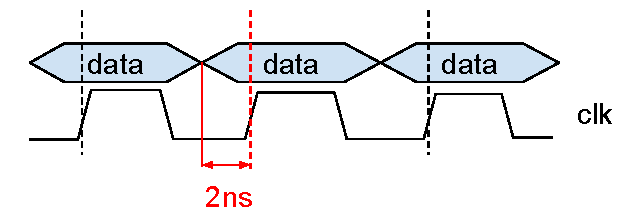
\includegraphics[width=0.8\textwidth]{slides/networking-driver-phy/rgmii_delays.pdf}
		\end{center}
\end{frame}

\begin{frame}{RGMII modes}
		\begin{columns}
		\column{0.4\textwidth}
			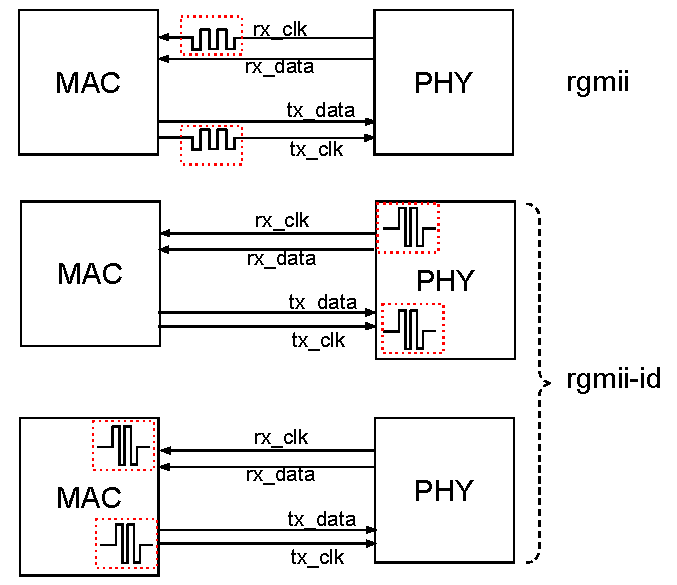
\includegraphics[width=1.2\textwidth]{slides/networking-driver-phy/rgmii_modes.pdf}
		\column{0.6\textwidth}
			\begin{itemize}
			\item The delays can be added using different methods :
			\item Longer PCB lines for the clock
				\begin{itemize}
					\item Very rarely done
				\end{itemize}
			\item Most PHYs and some MACs can insert delays internally
				\begin{itemize}
					\item RGMII-\textbf{ID} modes : \textbf{I}nternal \textbf{D}elay
					\item Preferred solution, delays are adjustable
				\end{itemize}
			\item Delays may only need to be added in one direction
				\begin{itemize}
					\item RGMII-TXID : TX delays are internal
					\item RGMII-RXID : RX delays are internal
				\end{itemize}
			\item Some MAC and PHYs have \textbf{hardwired} delays
			\end{itemize}
		\end{columns}
\end{frame}

\begin{frame}{RGMII modes in devicetree}
	\begin{itemize}
			\item \code{phy-mode} in devicetree : Hardware representation
				\begin{itemize}
					\item \textbf{\code{phy-mode = "rgmii";}} : No delays needs to be added
					\item \textbf{\code{phy-mode = "rgmii-id";}} : delays need to be added internally
					\item \textbf{\code{phy-mode = "rgmii-txid";}} : delays need to be added in TX
					\item \textbf{\code{phy-mode = "rgmii-rxid";}} : delays need to be added in RX
				\end{itemize}
			\item Internally, these mode are represented as \code{PHY_INTERFACE_MODE_RGMII[_ID|_TXID|_RXID]}
			\item The MAC driver reads the mode, and passes it to the PHY driver
			\item If the MAC inserts delays, it modifies the mode passed to the PHY
				\begin{enumerate}
					\item e.g. \code{phy-mode = "rgmii-id";}
					\item MAC inserts delays in TX, but not in RX
					\item MAC passes \code{PHY_INTERFACE_MODE_RXID} to the PHY
				\end{enumerate}

		\end{itemize}
\end{frame}

\begin{frame}{MDI - Media Dependent Interface}
	\vspace{3cm}
	\hfill
	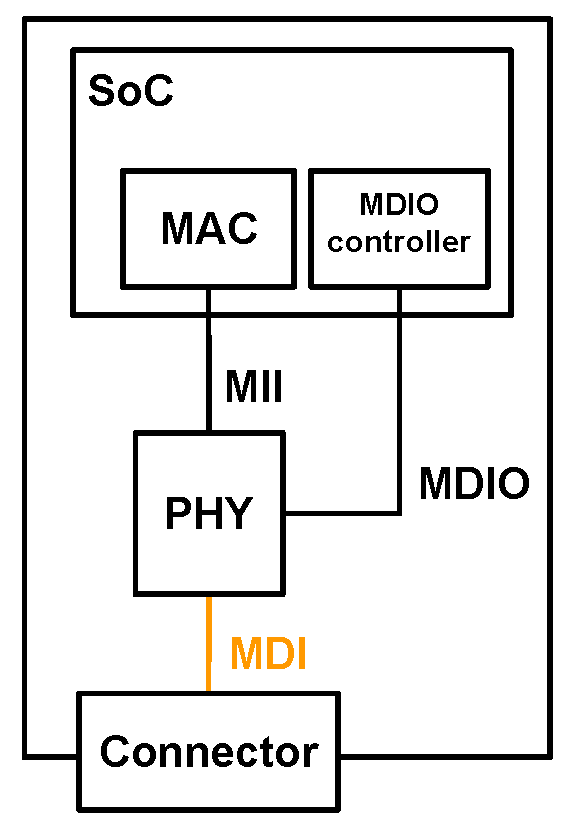
\includegraphics[width=0.15\textwidth]{slides/networking-driver-phy/mdi.pdf}
	\vspace{-6cm} % I'm sorry
	\begin{itemize}
		\item A huge number of physical protocols are defined by the 802.3 standard 
		\item As of v6.15, \href{https://elixir.bootlin.com/linux/v6.15.1/source/include/uapi/linux/ethtool.h\#L1950}{120} linkmodes are supported
		\item They follow a specific naming convention from IEEE 802.3
			    \item
{\color{blue}speed}\code{Band-}{\color{violet}Medium}{\color{red}Encoding}{\color{orange}Lanes}
: {\color{blue}1000}Base-{\color{violet}T},
{\color{blue}10G}Base-{\color{violet}K}{\color{red}R},
{\color{blue}10}Base-{\color{violet}T}{\color{orange}1}\dots
  \end{itemize}

  \begin{itemize}
    \item Band: \code{BASE}band, \code{BROAD}band or \code{PASS}band.
    \item {\color{violet}Medium}
      \begin{itemize}
        \item Base-\textbf{T}: Link over twisted-pair copper cables
(Classic RJ45).
	\item Base-\textbf{K}: Backplanes (PCB traces) links.
	\item Base-\textbf{C}: Copper links.
	\item Base-\textbf{L}, Base-\textbf{S}, Base-\textbf{F}: Fiber
        links.
	\item Base-\textbf{H}: Plastic Fiber.
      \end{itemize}
    \item {\color{red}Encoding}: Describe the block encoding used by the \code{PCS}
      \begin{itemize}
        \item Base-\textbf{X}: 10b/8b encoding.
	\item Base-\textbf{R}: 66b/64b encoding.
      \end{itemize}
    \item {\color{orange}Lanes}: Number of lanes per link (for
    Base-\textbf{T}, number of twisted pairs used).
	\end{itemize}
\end{frame}

\begin{frame}{linkmodes}
	\begin{itemize}
		\item In 802.3 Clauses 22 and 45, standard registers report the capabilities
		\item Allows dynamically building the list of MDI modes supported by the PHY
		\item Done in \kfunc{genphy_read_abilities} and \kfunc{genphy_c45_pma_read_abilities}
		\item PHY drivers can implement their own \code{phy_driver.get_features()}
		\item Get the supported linkmodes \textbf{on the interface} : \code{ethtool eth0}
			\begin{itemize}
				\item Intersection between :
				\item what the PHY can do : \code{phydev->supported}
				\item what the MAC can do based on the \textbf{mac capabilities}
				\item what the in-use \textbf{MII} interface can convey
			\end{itemize}
		\item The \textbf{advertised} linkmodes take into account the user settings
	\end{itemize}
\end{frame}

\begin{frame}{Interactions between MAC and PHY drivers}
	\begin{itemize}
		\item \textbf{phylib} provides an simple API for PHY consumers
			\begin{itemize}
				\item \kfunc{phy_start}, \kfunc{phy_stop}, \kfunc{phy_connect}
				\item \kfunc{phy_suspend}, \kfunc{phy_resume} for power management
			\end{itemize}
		\item MAC drivers may use that API, however it has some limitations :
			\begin{itemize}
				\item It can't handle MII reconfiguration
				\item It introduces some layering violations : MAC driver access \code{phydev->*} fields
				\item It makes it difficult to support other Layer 1 technologies such as \textbf{SFP}
			\end{itemize}
		\item \href{https://elixir.bootlin.com/linux/v6.15.1/source/drivers/net/phy/phylink.c}{phylink} is a framework that sits between MAC drivers and PHY drivers
		\item It abstracts away the PHY from the MAC, and provides a feature-full set of callbacks for MAC configuration
		\item It also handles PCS configuration

	\end{itemize}
\end{frame}

\begin{frame}{phylib usage in MAC drivers}
	\begin{itemize}
		\item MAC drivers that use \textbf{phylib} directly call \kfunc{phy_connect} to link with the PHY
			\begin{itemize}
				\item Their \code{.ndo_open()} calls \kfunc{phy_start} to establish the link
				\item Their \code{.ndo_close()} calls \kfunc{phy_stop} to quiesce it
			\end{itemize}
		\item They register an \code{.adjust_link} callback to the \code{phydev} for link change notification
	\end{itemize}
	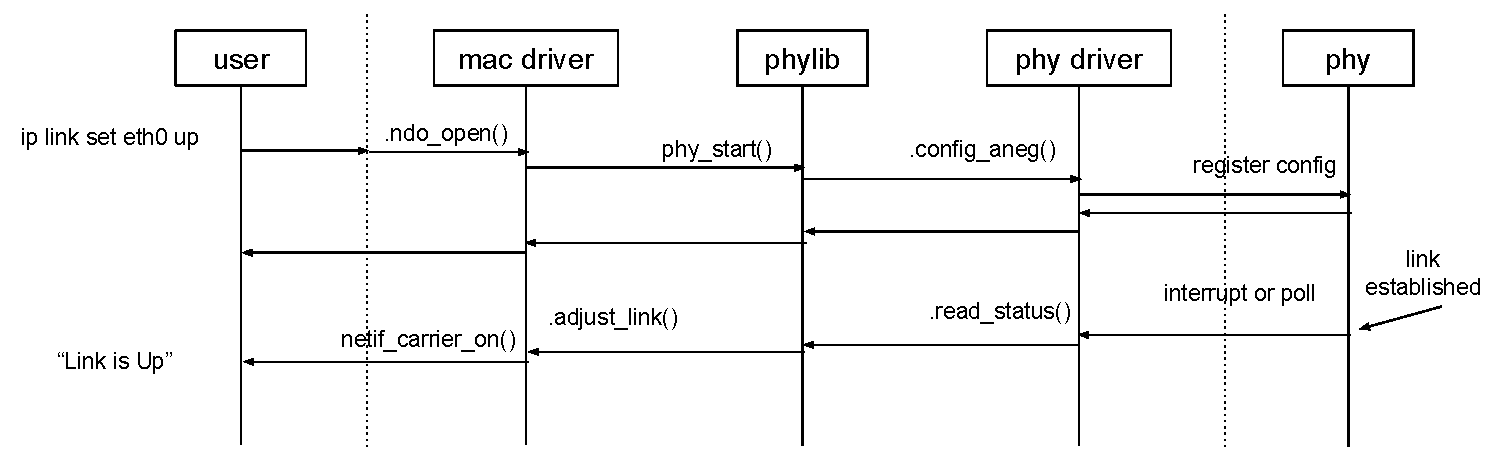
\includegraphics[width=\textwidth]{slides/networking-driver-phy/phylib_seq.pdf}
\end{frame}

\begin{frame}{phylink}
	\begin{itemize}
		\item The phylink framework abstracts the Layer 1 configuration away
		\item MAC driver can transparently connect to a PHY or an SFP module
		\item Handles MII reconfiguration, PCS configuration, ethtool reconfiguration
		\item Doesn't superseeds phylib, but complements it for the MAC API
	\end{itemize}
	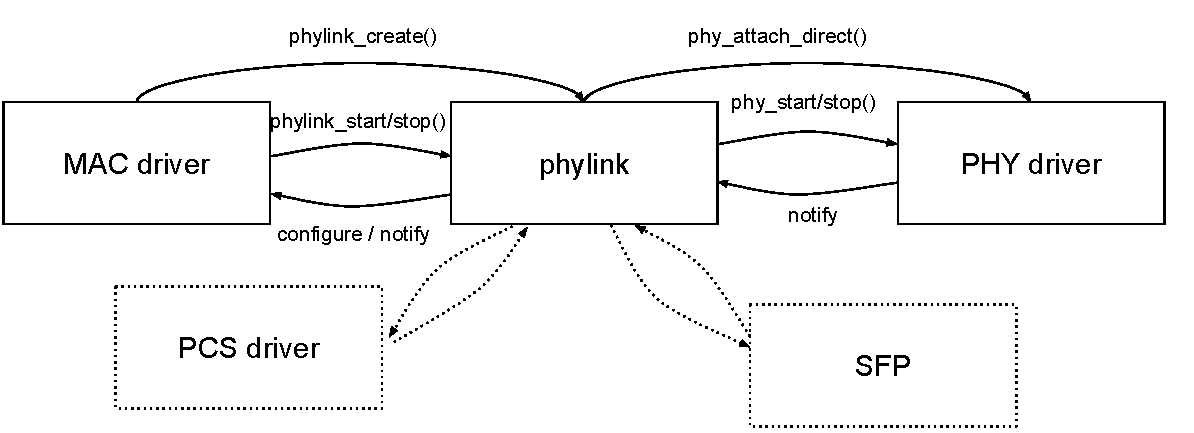
\includegraphics[width=\textwidth]{slides/networking-driver-phy/phylink.pdf}
\end{frame}

\begin{frame}[fragile]{phylink - MAC ops}
	\begin{itemize}
		\item MAC driver populate a set of callbacks in \kstruct{phylink_mac_ops} registered to phylink
		\item \code{.mac_config} : Reconfigure the \textbf{MII} mode and parameters, \textbf{major reconfig}
		\item \code{.mac_link_up} : Notify that the link with the partner is established
			\begin{itemize}
				\item Negociated speed, duplex and flow control are passed
				\item The MAC should re-adjust its settings, if possible without bringing the link down
			\end{itemize}
		\item \code{.mac_link_down} : Notify that the link partner is gone
		\item \code{.mac_select_pcs} : The MAC returns which \kstruct{phylink_pcs} must be used
			\begin{itemize}
				\item MACs may have \href{https://elixir.bootlin.com/linux/v6.15.1/source/drivers/net/ethernet/marvell/mvpp2/mvpp2_main.c\#L6468}{multiple PCS}, chosen based on the MII
			\end{itemize}
		\item \code{.mac_enable/disable_tx_lpi} : Configures the \textbf{Low Power Idle} modes, for \textbf{E}nergy \textbf{E}fficient \textbf{E}thernet
	\end{itemize}
\end{frame}

\begin{frame}[fragile]{phylink - MAC capabilities}
	\begin{itemize}
		\item When creating the \kstruct{phylink} instance, the MAC indicates its capabilities
		\item This is done by populating a \kstruct{phylink_config} object
		\item \code{mac_capabilities} : indicates all Speeds and Duplex settings supported
		\item \code{supported_interfaces} : indicates all MII interfaces this MAC can output
	\end{itemize}
	\begin{block}{phylink config example}
	{\fontsize{9}{10}
	\begin{minted}{c}
phylink_config.mac_capabilities = MAC_ASYM_PAUSE | MAC_SYM_PAUSE | MAC_10 |
                                  MAC_100 | MAC_1000FD | MAC_2500FD;
phy_interface_set_rgmii(phylink_config.supported_interfaces);
__set_bit(PHY_INTERFACE_MODE_MII, phylink_config.supported_interfaces);
__set_bit(PHY_INTERFACE_MODE_GMII, phylink_config.supported_interfaces);
__set_bit(PHY_INTERFACE_MODE_SGMII, phylink_config.supported_interfaces);
__set_bit(PHY_INTERFACE_MODE_1000BASEX, phylink_config.supported_interfaces);
__set_bit(PHY_INTERFACE_MODE_2500BASEX, phylink_config.supported_interfaces);
	\end{minted}
	}
	\end{block}
\end{frame}

\begin{frame}{SFP}
	\begin{itemize}
		\item \textbf{S}mall \textbf{F}ormfactor \textbf{P}luggable is defined by the SFF standards
		\item It allows having a hot-pluggable \textbf{module} that deals with the Media side
		\item Useful for \textbf{Fibre} links, but also exists in Copper flavours (BaseT or DAC)
		\item Each module has a standardized behaviour and interface :
			\begin{itemize}
				\item An \textbf{i2c} bus and some GPIOs are used to control the module
				\item An \textbf{eeprom} is accessible on the \textbf{i2c} bus, at address \code{0x50}
				\item Its content is standardized, indicating the capabilities, vendor, model, etc.
				\item Some modules also provide Diagnostics and Montoring over i2c : Temperature, Power output, etc.
			\end{itemize}
	\end{itemize}
\end{frame}

\begin{frame}{SFP}
	\begin{itemize}
		\item The internals of an SFP module are a black box, but some modules may have a PHY within
		\item The PHY may be accessed over the i2c bus, but not always
		\item If accessible, the embedded PHY can be managed by the kernel
		\item If the SoC can't output a \textbf{serialized} interface, a \textbf{media converter} can be used
	\end{itemize}
	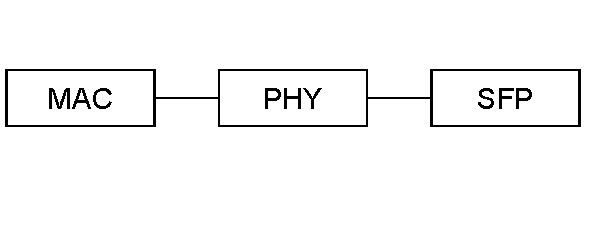
\includegraphics[width=0.6\textwidth]{slides/networking-driver-phy/phy_sfp.pdf}
\end{frame}

\begin{frame}{Ethtool reporting}
	\begin{itemize}
		\item Userspace can retrieve information reported by the PHY drivers through \code{ethtool}
		\item Contrary to \kstruct{net_device}, \kstruct{phy_driver}s don't implement \code{ethtool ops}
		\item \code{phylib} implements the \kstruct{ethtool_phy_ops}, and calls into \kstruct{phy_driver}
		\item The netdev \code{ethtool_ksettings_get} and \code{ethtool_ksettings_set} have PHY-centric implementation :
			\begin{itemize}
				\item They report the current link settings : Speed, duplex, linkmodes
				\item Also report Link-partner information : The \textbf{advertised} linkmodes 
				\item See \kfunc{phylink_ethtool_ksettings_set} and \kfunc{phy_ethtool_ksettings_set}
			\end{itemize}
	\end{itemize}
\end{frame}

\begin{frame}{PHY reporting with Netlink}
	\begin{columns}
		\column{0.2\textwidth}
		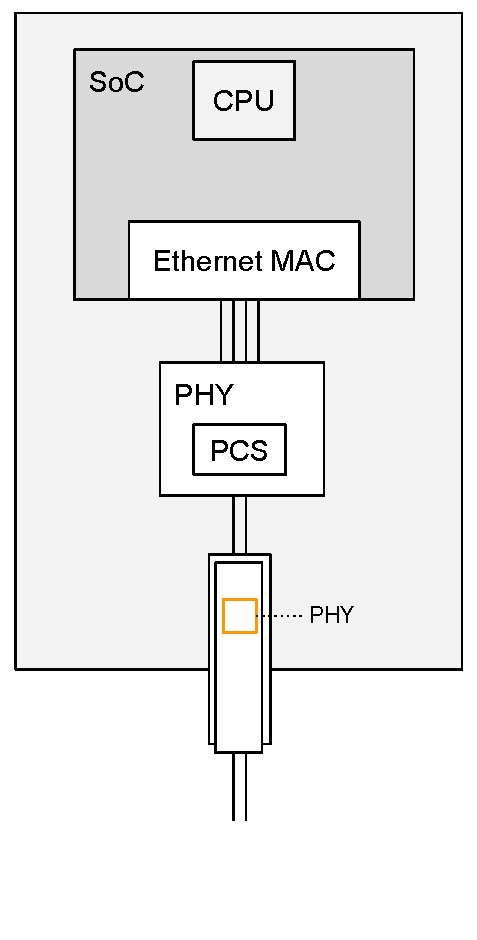
\includegraphics[width=0.9\textwidth]{slides/networking-driver-phy/one-media-converter-one-phy-one-mac.pdf}
		\column{0.8\textwidth}
	\begin{itemize}
		\item Some hardware topologies may have \textbf{more than one PHY} attached to a MAC
			\begin{itemize}
				\item When an SFP module is driven by a PHY, and contains a PHY itself
				\item When a PHY is used as a \textbf{media converter}
			\end{itemize}
		\item Netlink requests targetting PHY devices can now be passed a \textbf{phy index}
			\begin{itemize}
				\item Implemented by \kfile{drivers/net/phy/phy_link_topology.c}
			\end{itemize}
	\end{itemize}
	\end{columns}
\end{frame}

% MDIO bus and PHY devices
% phydev and phylib
% phylink, PCS
% sfp
% linkmodes, ksettings, autoneg

